\chapter{Nucleon Decay and Atmospheric Neutrinos}
\label{ch:physics-atmpdk}

\section{Nucleon Decay}
\label{sec:physics-atmpdk-ndk}

\subsection{Physics Motivation}
	The class of theories known as Grand Unified Theories (GUTs) make
predictions about both baryon number violation and  proton lifetime that may be
within reach of the full-scope DUNE experiment. 
%
The theoretical motivation for the study of proton decay has a long and
distinguished history~\cite{Pati:1973rp,Georgi:1974sy,Dimopoulos:1981dw} and
has been reviewed many times~\cite{Langacker:1980js,deBoer:1994dg,Nath:2006ut}.
%
Early GUTs provided the original motivation for proton decay searches in
kiloton-scale detectors placed deep underground to limit backgrounds.  The
\ktadj{22.5} \superk\ experiment extended the search for proton decay by more
than an order of magnitude relative to the previous generation of experiments.
%
Contemporary reviews~\cite{Raby:2008pd,Senjanovic:2009kr,Li:2010dp} discuss the
strict limits already set by \superk\ and the context of the proposed next
generation of larger underground
%\SI{100}{\kt}-scale 
experiments such as Hyper-Kamiokande and DUNE.

Although no evidence for proton decay has been detected, the lifetime
limits from the current generation of experiments already constrain
the construction of many contemporary GUT %theoretical 
models. In some cases, these lifetime limits are approaching the upper limits
allowed
by GUT models.
%Indeed,
%a tension between the limits imposed by current experiments and those
%still allowed by theory is now commonly discussed. \fixme{I still think the
%nature of the 'tension'
%requires some explanation} 
This situation points naturally toward continuing the search with new, larger
detectors.
%These searches are motivated by a range of scientific issues:
%\begin{itemize}
%\item Conservation laws arise from underlying symmetries in
%Nature~\cite{Noether:1918zz}.  
%  Conservation of baryon number is therefore
%  unexplained since it corresponds to no known long-range force or
%  symmetry.
%\item Baryon number non-conservation has cosmological consequences,
%  such as a role in inflation and the matter-antimatter asymmetry of the
%  Universe.
%\item Proton decay is predicted at some level by almost all GUTs. 
%\item Some GUTs can accommodate
%  neutrinos with nonzero mass and characteristics consistent with
%  experimental observations.
%\item GUTs incorporate other previously unexplained features of
%  the Standard Model such as the relationship between quark and lepton
%  electric charges. 
%\item The unification scale is suggested both experimentally and
%  theoretically by the apparent convergence of the running coupling
%  constants of the Standard Model. The unification scale is in excess of
%\SI{e15}{GeV}.%$10^{15}$~GeV.
%\item The unification scale is not accessible by any accelerator
%  experiment; it can only be probed by virtual processes such as with
%  proton decay.
%\item GUTs usually predict the relative branching
%  fractions of different nucleon decay modes. Testing these predictions
%  would, however, require a sizeable sample of proton decay events.
%\item The dominant proton decay mode of a GUT is often sufficient to roughly
%  identify the likely characteristics of the GUT,
%  such as gauge mediation or the involvement of supersymmetry.
%\end{itemize}
\subsection{Proton Decay Modes} 

\tikzset{
particle/.style={draw=blue, postaction={decorate},
    decoration={markings,mark=at position .6 with {\arrow[blue]{triangle
45}}}},
noarrow/.style={draw=blue},
boson/.style={draw=blue,dashed},
}

\begin{figure}[!htb]
  \begin{center}
\begin{tikzpicture}
  \coordinate (cross);
  \coordinate[above left=of cross, label={[yshift=-6mm]$d$}](d);
  \coordinate[below left=of cross, label={[yshift=1mm]$u$}](u);  
  \coordinate[above right=of cross](tau);
  \coordinate[below right=of cross](tee);
  \coordinate[right=of tau, label=below:$\overline{\nu}_\tau$] (vtau);
  \coordinate[right=of tee, label=above:$\overline{s}$] (sbar);
  \coordinate[below=of u, label=above:$u$](u2);
  \coordinate[below=of sbar, label=above:$u$](u3);

  \draw[particle] (d) -- (cross);
  \draw[particle] (u) -- (cross);
  \draw[noarrow] (cross) -- node[label=above left:$\widetilde{\tau}$] {} (tau);
  \draw[noarrow] (cross) -- node[label=below left:$\widetilde{t}$] {} (tee);
  \draw[boson] (tau) -- node[label=right:$\widetilde{W}$] {} (tee);
  \draw[particle] (vtau) -- (tau);
  \draw[particle] (sbar) -- (tee);
  \draw[particle] (u2) -- (u3);

  \draw [decorate,decoration={brace,mirror,raise=3mm}] (d) -- (u2) node
[black,midway,xshift=-8mm] {$P$};
  \draw [decorate,decoration={brace,raise=3mm}] (sbar) -- (u3) node
[black,midway,xshift=8mm] {$K^+$};

\end{tikzpicture}%
%\begin{tikzpicture}
\begin{tikzpicture}
  \coordinate (x);
  \coordinate[above left=of x, label={[yshift=-5mm]$u$}](u);
  \coordinate[below left=of x, label={[yshift=1mm]$u$}](u2);  
  \coordinate[right=of x](x2);  
  \coordinate[above right=of x2, label={[yshift=-6mm]$e^+$}](eplus);  
  \coordinate[below right=of x2, label={[yshift=1mm]$\overline{d}$}](dbar);
  \coordinate[below=of u2,label=above:$d$](d);  
  \coordinate[below=of dbar, label=above:$d$](d2);  

  \draw[particle] (u) -- (x);
  \draw[particle] (u2) -- (x);
  \draw[boson] (x) -- node[label=above:$X$] {} (x2);
  \draw[particle] (eplus) -- (x2);
  \draw[particle] (dbar) -- (x2);
  \draw[particle] (d) -- (d2);

  \draw [decorate,decoration={brace,mirror,raise=3mm}] (u) -- (d) node
[black,midway,xshift=-8mm] {$P$};
  \draw [decorate,decoration={brace,raise=3mm}] (dbar) -- (d2) node
[black,midway,xshift=8mm] {$\pi^0$};

\end{tikzpicture}
  \end{center}
%\centerline{
%\includegraphics[width=0.5\textwidth]{pepi0_feyn.jpg}
%\includegraphics[width=0.5\textwidth]{pknu_feyn.png}
%}
\caption[Proton decay modes from SUSY and gauge-mediation models]{Feynman
diagrams for proton decay modes from
supersymmetric GUT, $p^+ \rightarrow K^+ \overline{\nu}$  (left) and
gauge-mediation GUT models, $p^+ \rightarrow e^+ \pi^0$ (right).}
\label{pdk_feyn}
\end{figure}
From the body of literature, two decay modes (shown in Figure~\ref{pdk_feyn})
emerge that dominate the DUNE experimental design. The more
well-known of the two, the decay mode of $p \rightarrow e^+ \pi^0$,
arises from gauge mediation.  It is often predicted to have the higher
branching fraction and is also demonstrably the more straightforward
experimental signature for a water Cherenkov detector. In this mode,
the total mass of the proton is converted into the electromagnetic
shower energy of the positron and two photons from $\pi^0$ decay,
with a net momentum vector near zero. 

The second key mode is $p \rightarrow K^+ \overline{\nu}$.  This mode is
dominant in most supersymmetric GUTs, many of which also favor additional modes
involving kaons in the final state. This decay mode with a charged kaon is
uniquely interesting; since stopping kaons have a higher ionization density
than other particles, a LArTPC could detect it with extremely high efficiency.
In addition, many final states of $K^+$ decay would be fully reconstructable in
a LArTPC.

There are many other allowed modes of proton or bound neutron into
antilepton plus meson decay that conserve $B-L$\footnote{In these
  models, the quantum number $B-L$ is expected to be conserved even
  though $B$ and $L$ are not individually conserved.}. 
%but none of
%these will influence the design of a next-generation experiment. 
%The
%most stringent limits, besides those on $p \rightarrow e^+ \pi^0$,
%include the lifetime limits on $p \rightarrow \mu^+ \pi^0$ and $p
%\rightarrow e^+ \eta$, both of which are greater than \num{4e33} 
%years~\cite{Nishino:2012ipa}. Any experiment that will do well for $p
%\rightarrow e^+ \pi^0$
%will also do well for these decay modes.  The decays $p \rightarrow
%\overline\nu \pi^+$ or $n \rightarrow \overline\nu \pi^0$ may have
%large theoretically predicted branching fractions, but they are
%experimentally difficult due to the sizeable backgrounds from
%atmospheric-neutrino interactions. The decay $p \rightarrow \mu^+ K^0$
%can be detected relatively efficiently by either water Cherenkov or
%LArTPC detectors.
Other modes that conserve $B+L$, or that decay only into leptons,  
have also been hypothesized. 
%that violate only baryon number, or that decay
These possibilities are less well-motivated theoretically, as
they do not appear in a wide range of models, and are therefore not considered
here.

Figure~\ref{PDK-limits-theory} shows a comparison of experimental
limits, dominated by recent results from \superk\ to the
ranges of lifetimes predicted by an assortment of GUTs. At this time,
the theory literature does not attempt to precisely predict lifetimes,
concentrating instead on suggesting the dominant decay modes and
relative branching ratios. The uncertainty in the lifetime
predictions comes from details of the theory, such as masses and
coupling constants of unknown heavy particles, as well as poorly known
details of matrix elements for quarks within the nucleon.

\begin{cdrfigure}[Proton decay lifetime limits  compared to lifetime ranges
  predicted by GUTs]{PDK-limits-theory}{Proton decay lifetime
limits~\cite{Beringer:1900zz,Nishino:2012ipa} compared to lifetime ranges
  predicted by Grand Unified Theories. The upper section is for
  $p \rightarrow e^+ \pi^0$, most commonly caused by gauge mediation.
  The lower section is for SUSY-motivated models, which commonly
  predict decay modes with kaons in the final state. The
  marker symbols indicate published experimental limits, as indicated
  by the sequence and colors on top of the figure.}
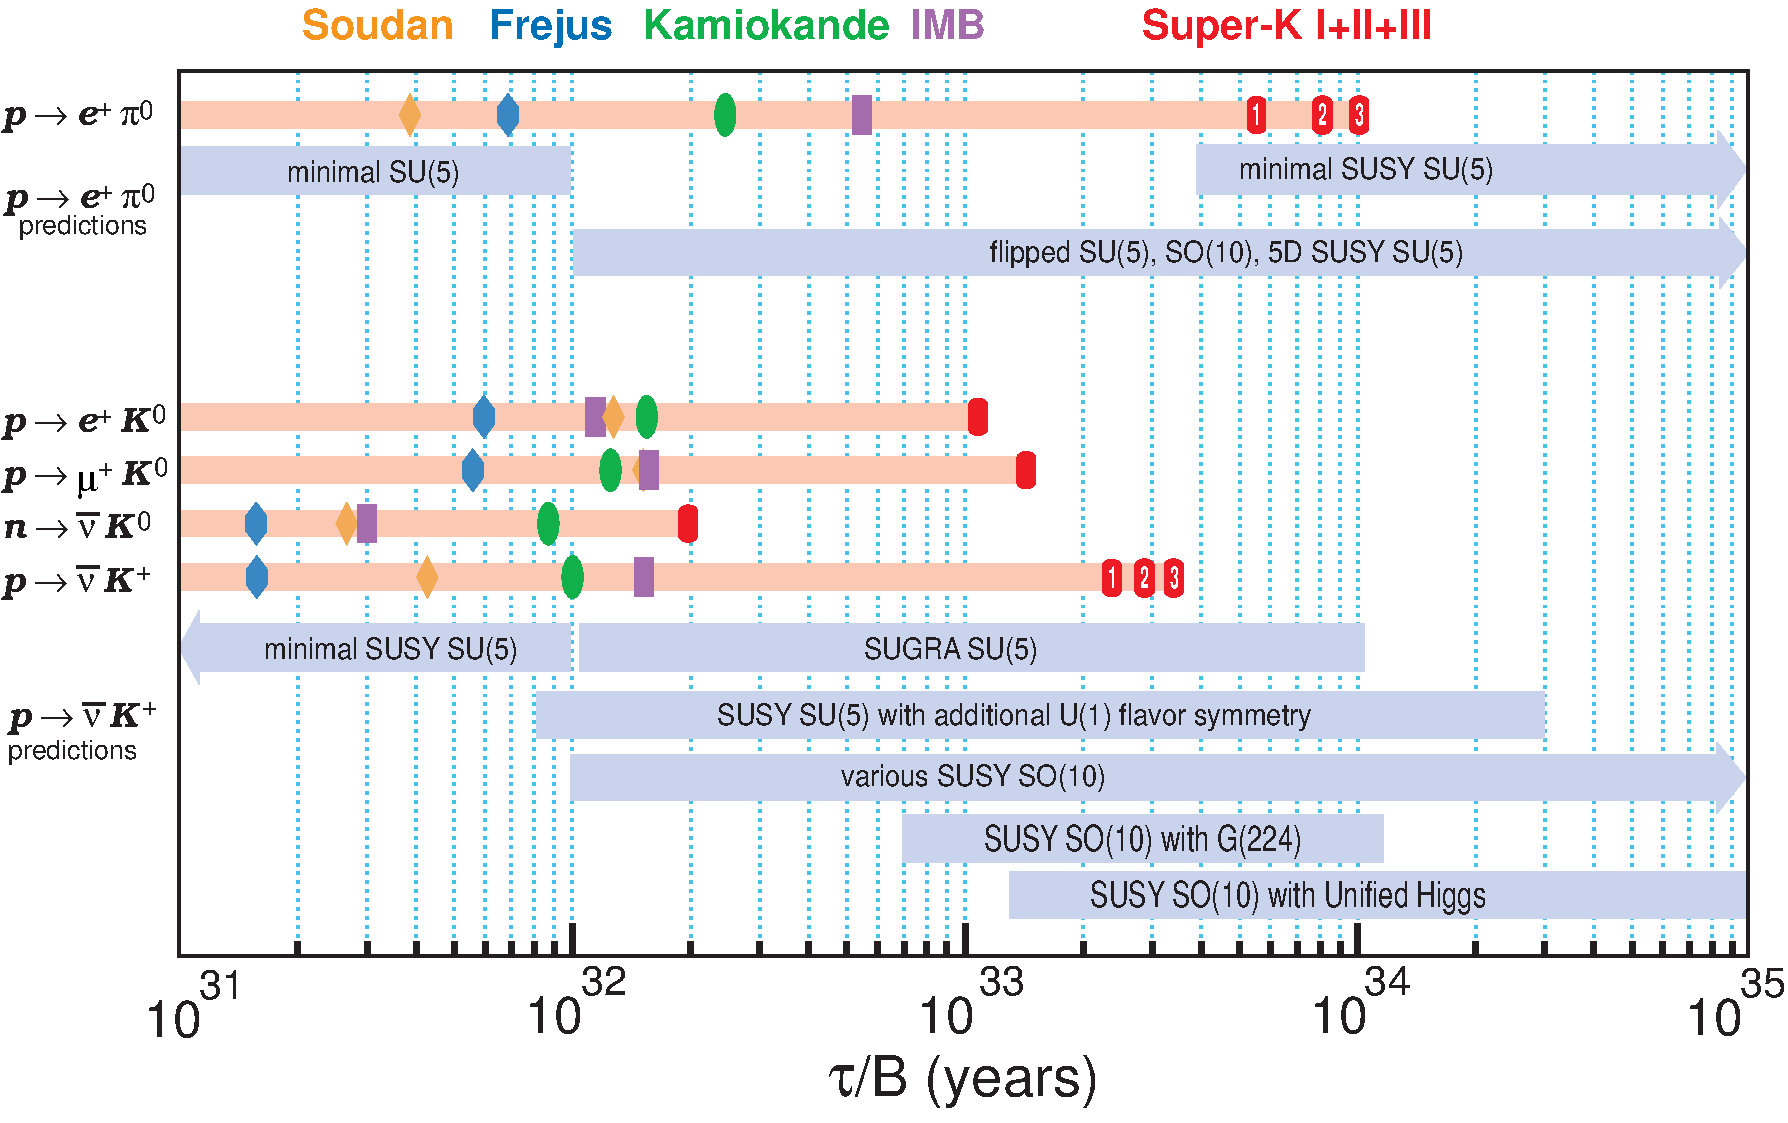
\includegraphics[width=0.9\textwidth]{PDK-limits-theory_fix.pdf}
\end{cdrfigure}


It is apparent from Figure~\ref{PDK-limits-theory} that a continued
search for proton decay is by no means assured of obtaining a positive
result.  With that caveat, an experiment with sensitivity to proton lifetimes
between $10^{33}$ and $10^{35}$ years is searching in the right territory over
virtually all GUTs; even if no proton decay is detected,
stringent lifetime limits will provide strong constraints on such
models.  Minimal SU(5) was ruled out by the early work of IMB and
Kamiokande and minimal SUSY~SU(5) is considered to be ruled out by \superk.
In most cases, another order of magnitude in improved limits will not rule out
specific models but will constrain their allowed parameters;
this could allow identification of models which must be fine-tuned
in order to accommodate the data, and are thus less favored.

%%%%%%%%%%%%%%%%%%%%%%%%%%%%%%%%%%%%%%%%%%%%%%%%%%%%%%%%%%%%%%%%
%\subsection{DUNE Sensitivity to Proton Decay}

%Current limits on nucleon decay via numerous channels are dominated by
%\superk\ (SK)~\cite{Raaf:2012pva}, for which the most recently
%reported preliminary results are based on an overall exposure of
%\SI{260}{\ktyr}.
%
%Although the SK search has so far not observed nucleon decay, it
%has established strict limits ($90\%$ CL) on the partial lifetimes for
%decay modes of particular interest to GUT models such as $\tau/B(p\to
%e^+\pi^0) > 1.3\times 10^{\mathrm{34}}\,$year and $\tau/B(p\to
%K^+\overline{\nu}) > 0.59\times
%10^{\mathrm{34}}\,$year~\cite{kearns_isoups}.  These are significant
%limits on theoretical models that constrain model builders and set a
%high threshold for the next-generation detectors such as DUNE and
%Hyper-Kamiokande (Hyper-K). After more than ten years of exposure, the SK limits
%will improve only slowly. A much more massive detector such as
%Hyper-K --- which will have a \ktadj{560} fiducial mass 
%--- is required to make a significant (order-of-magnitude) improvement 
%using the water Cherenkov technique.

%The uniqueness of proton decay signatures in a
%LArTPC and the potential for reconstructing them with redundant information has
%long been recognized as a key strength of this technology. A LArTPC can
%reconstruct all final-state charged particles and make an accurate assessment of
%particle type, distinguishing between muons, pions, kaons and protons.
%Electromagnetic showers are readily measured, and those that originate from
%photons generated by $\pi^0$ decay can be distinguished to a significant degree
%from those that originate from $\nu_e$ charged-current (CC) interactions.
%%Kiloton-per-kiloton, LArTPC technology is expected to outperform water Cherenkov
%in both detection efficiency and atmospheric-neutrino background rejection for
%most nucleon decay modes, although intranuclear effects, which can smear out
%some of the proton decay signal, are smaller for oxygen and nonexistent for
%hydrogen.

%When mass and cost are taken into account, water Cherenkov technology
%is optimum for the $p\to e^+\pi^0$ final-state topology, where the
%signal efficiency is roughly 40\% and the background rate is two events per
%\SI{}{\Mtyr}.  The efficiency estimate for this mode~\cite{Bueno:2007um} for a
%LArTPC is 45\% with one event per  \SI{}{\Mtyr} --- not a significant enough
%improvement in efficiency to overcome the penalty of the higher cost per kiloton
%for liquid argon.

%For the $p \rightarrow K^+ \overline{\nu}$ in a LArTPC, the $K^+$ track can be
%reconstructed and uniquely identified as a charged kaon, leading to exceptional
%background rejection. The efficiency for the $K^+ \overline{\nu}$ mode in a
%LArTPC is estimated to be as high as 97.5\% with a background rate of one event
%per \SI{}{\Mtyr}. 
%%In water Cherenkov detectors the efficiency for this mode is roughly
%%19\% for a low-background search, with a background rate of four events
%%per  \SI{}{\Mtyr}.
%Based on these numbers and a ten-year exposure, DUNE's 
%\ktadj{40} LArTPC and the \ktadj{560} Hyper-K WCD have comparable
%sensitivity (at 90\% CL), but the estimated LArTPC background of 0.3
%events is dramatically better than the 22 estimated for Hyper-K 
%(assuming no further improvement in analysis technique past that
%currently executed for SK~\cite{kearns_isoups}).
 
%%%%%%%%%%%%%%%%%%%%%%%%%%%%%%%%%%%%%%%%%%%%%%%%%%%%%%%%%%%%%%%%
%%%%%%%%%%%%%%%%%%%%%%%%%%%%%%%%%%%%%%%%%%%%%%%%%%%%%%%%%%%%%%%%
\subsection{Signatures for Nucleon Decay in Liquid Argon}

For modes with no
electron in the final state, the same displaced vertex performance
that underpins long-baseline neutrino oscillation measurements allows
the rejection of CC interactions of atmospheric $\nu_e$'s.
As will be stressed for the key mode of $p \rightarrow K^+ \overline{\nu}$
described in detail below, the capability to reconstruct the charged
kaon with the proper range and $dE/dx$ profile allows for a high-efficiency,
background-free analysis.  In general, these criteria favor all
modes with a kaon, charged or neutral, in the final state. Conversely,
the efficiency for decay modes to a lepton plus light meson will be
limited by intranuclear reactions that plague liquid argon to a greater extent
than they do $^{\mathrm{16}}$O in a water Cherenkov detector.

An extensive survey~\cite{Bueno:2007um} of nucleon decay efficiency 
and background rates for large LArTPCs with various depth/overburden 
conditions, published in 2007, provides the starting point for the 
assessment of DUNE's capabilities.  Table~\ref{tab:pdecay} lists selected
modes where LArTPC technology exhibits a significant performance 
advantage (per kiloton) over the water Cherenkov technology.
The remainder of this chapter focuses on the capabilities 
of DUNE for the $p\to K^+\overline{\nu}$ channel, as the most 
promising from theoretical and experimental 
considerations.  Much of the discussion that follows can be 
applied to cover the other channels with kaons listed in 
the table.
%
\begin{table}[!htbp]
\caption[Efficiencies and background rates for nucleon decay modes]
        {Efficiencies and background rates (events per \SI{}{\Mtyr}) for nucleon decay 
         channels of interest for a large underground LArTPC~\cite{Bueno:2007um}, and 
         comparison with water Cherenkov detector capabilities.  
         The entries for the water Cherenkov capabilities are based 
         on experience with the \superk{} detector~\cite{kearns_isoups}.  
        }
\begin{center}
\begin{tabular}{$L^c^c^c^c} %$ 
\toprule
\rowtitlestyle
Decay Mode   & \multicolumn{2}{^>{}c}{Water Cherenkov} & 
\multicolumn{2}{^>{}c}{Liquid Argon TPC} \\
\rowtitlestyle
   & Efficiency &   Background & Efficiency &   Background \\ \toprowrule
$p \rightarrow K^+ \overline{\nu}$       & 19\%  &  4   &  97\%   &     1  \\ \colhline
$p \rightarrow K^0 \mu^+$      & 10\%  &  8   &  47\%   &  $<2 $ \\ \colhline
$p \rightarrow K^+ \mu^- \pi^+$ &       &      &  97\%   &     1  \\ \colhline
$n \rightarrow K^+ e^- $        & 10\%  &  3   &  96\%   &  $<2$  \\ \colhline
$n \rightarrow e^+\pi^-$      & 19\%  &  2   &  44\%   &  0.8   \\
\bottomrule
\end{tabular}
\end{center}
\label{tab:pdecay}
\end{table}
%

The key signature for $p\to K^+\overline{\nu}$ is the presence of an
isolated charged kaon (which would also be monochromatic 
for the case of free protons, with $p=$\SI{340}{\MeV}).  
Unlike the case of $p\to e^+\pi^0$, where the maximum
detection efficiency is limited to 40--45\% because of inelastic
intranuclear scattering of the $\pi^0$, the kaon in $p\to
K^+\overline{\nu}$ emerges intact (because the kaon momentum is 
below threshold for inelastic reactions)
from the nuclear environment of the decaying proton $\sim 97\%$ of the
time.  Nuclear effects come into play in other ways, however: the kaon
momentum is smeared by the proton's Fermi motion and shifted downward
by re-scattering~\cite{Stefan:2008zi}. 
%The kaon emerging from this process is below Cherenkov threshold,
%therefore a water detector would need to detect it after it stops, via its
%decay products.  
Not all $K$ decay modes are reconstructable, however,
and even for those that are, insufficient information exists to
determine the initial $K$ momentum.  Still, water detectors can
reconstruct significant hadronic channels such as $K^+\to\pi^+\pi^0$
decay, and the \MeVadj{6} gamma from de-excitation of $O^{16}$ provides an
added signature to help with the $K^+\to\mu^+\nu$ channel. The overall
detection efficiency in SK~\cite{kearns_isoups} thus approaches
$20\%$.

In LArTPC detectors, the $K^+$ can be tracked, its momentum measured
by range, and its identity positively resolved via detailed analysis
of its energy-loss profile.  Additionally, all decay modes can be
cleanly reconstructed and identified, including those with neutrinos,
since the decaying proton is essentially at rest.  With this level of
detail, it is possible for a single event to provide overwhelming
evidence for the appearance of an isolated kaon of the right momentum
originating from a point within the fiducial volume.  The strength of
this signature is clear from cosmogenic-induced kaons observed by the
ICARUS Collaboration in the cosmic-ray (CR) test run of half of the T600
detector, performed at a surface installation in Pavia~\cite{Amerio:2004ze} 
and in high-energy neutrino interactions with the full T600 in the recent 
CNGS (CERN Neutrinos to Gran Sasso) run~\cite{Antonello:2012hu}.
Figure~\ref{fig:icaruskaon} shows a sample event from the CNGS run in
which the kaon is observed as a progressively heavily-ionizing track 
that crosses into the active liquid argon volume, stops, and
decays to $\mu\nu$, producing a muon track that also stops and decays
such that the Michel-electron track is also visible. 
%The 3D
%reconstruction of the event is shown in Figure~\ref{fig:icarusk3d}.
%
\begin{figure}[!htb]
\centering
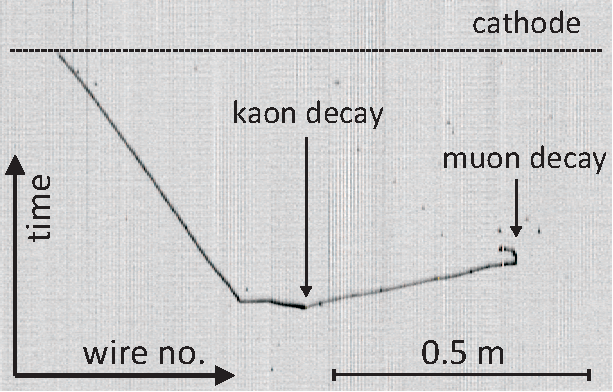
\includegraphics[width=0.72\textwidth]{Fig14a_kaon-coll_raw_R10599E8083.pdf}
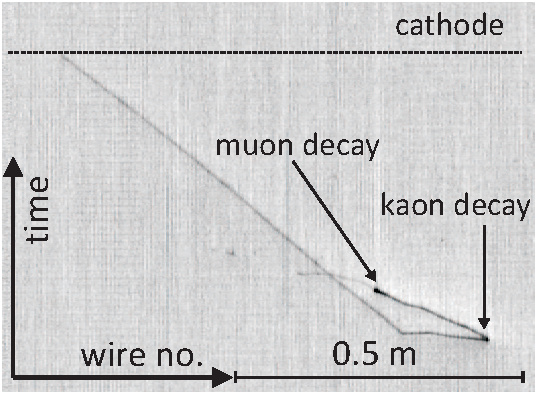
\includegraphics[width=0.72\textwidth]{Fig14b_kaon-ind2_raw_R10599E8083.pdf}
\caption[Decaying kaon observed during the ICARUS run at CNGS]
{Event display for a decaying kaon candidate $K \rightarrow \mu \nu_\mu \ \mu \rightarrow e \nu_e \nu_\mu$ 
in the ICARUS T600 detector observed
in the CNGS data ($K$: \SI{90}{\cm}, \SI{325}{\MeV}; $\mu$ : \SI{54}{\cm}, \SI{147}{\MeV}; 
$e$ : \SI{13}{\cm}, \SI{27}{\MeV}). The top figure shows the signal on the collection plane,
  and the bottom figure shows the signal on the second induction plane~\cite{Antonello:2012hu}.}
\label{fig:icaruskaon}
\end{figure}
%\begin{figure}[!htb]
%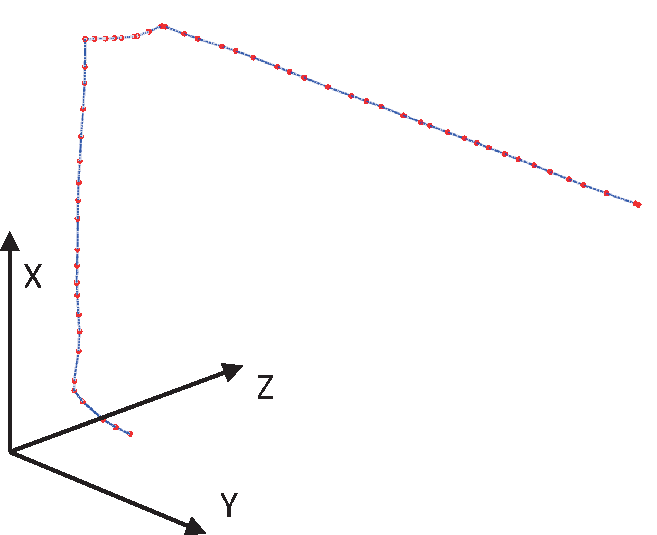
\includegraphics[width=0.7\textwidth]{Fig14c_new.pdf}
%\caption[3D construction of decaying kaon in the ICARUS detector]{3D reconstruction of the decaying kaon event observed in the ICARUS T600 detector and shown in Figure~\ref{fig:icaruskaon}.}
%\label{fig:icarusk3d}
%\end{figure}

If it can be demonstrated that background processes mimicking this
signature can be rejected at the appropriate level, 
a single $p\to K^+\overline{\nu}$ candidate could constitute 
evidence for proton decay. %The background rejection capability of the DUNE far detector is the topic of Section~\ref{sec:pdk:background-rej} below.

	Ref.~\cite{lbne-sciopp} presented a detailed examination of possible
backgrounds, including those arising from cosmic ray interactions in the
detector and surrounding rock, atmospheric neutrino interactions in the
dectector, and reconstruction failiures. Table~\ref{tab:pdkbkds} summarizes the
results of those background studies.
\begin{table}[!htbp]
\caption[Background Summary for Nucleon Decay]
        {Background rates (events per \SI{}{\Mtyr}) for nucleon decay }
%        {rates (events per \SI{}{\Mtyr}) for nucleon decay 
%         channels of interest for a large underground LArTPC~\cite{Bueno:2007um}, and 
%         comparison with water Cherenkov detector capabilities.  
%         The entries for the water Cherenkov capabilities are based 
%         on experience with the \superk{} detector~\cite{kearns_isoups}.  
%        }
\begin{center}
\begin{tabular}{$L^c^c} %$ 
\toprule
\rowtitlestyle
Background Source & Mitigation Strategy & Leakage Rate  \\
\rowtitlestyle
& & (events per \SI{}{\Mtyr})\\
\toprowrule
Internal cosmic ray spallation      & Energy threshold & Negligible  \\ \colhline
External cosmogenic & & \\
$K^+$ production  & Depth, fiducialization & Negligible \\ \colhline
External cosmogenic  & & \\
$K^0$ production & & \\
+internal charge-exchange  & & \\
to $K^+$ & Cuts on other secondaries &   2  \\ \colhline
Atmospheric $\nu$ & & \\ 
$\Delta S=0$ processes & Cut on associated strange baryon & Negligible   \\ \colhline
Atmospheric $\nu$ & Cabibo-suppressed, & \\ 
$\Delta S=1$ processes &lepton ID & Negligible \\ \colhline
Atmospheric $\nu$ & $dE/dx$ discrimination, & \\
with $\pi$ mis-ID & +236 MeV muon track & Negligible \\
\colhline
Reconstruction pathologies & $dE/dx$ profiles vs track length & Negligible \\
\colhline
\bottomrule
\end{tabular}
\end{center}
\label{tab:pdecay}
\end{table}
%

%%%%%%%%%%%%%%%%%%%%%%%%%%%%%%%%%%%%%%%%%%%%%%%%%%%%%%%%%%%%%%%%
%%%%%%%%%%%%%%%%%%%%%%%%%%%%%%%%%%%%%%%%%%%%%%%%%%%%%%%%%%%%%%%%
%\subsection{Background Levels and Rejection Capabilities}
%\label{sec:pdk:background-rej}
%
%This section discusses the key background processes and 
%their signatures, focusing on the $p\to K^+\overline{\nu}$ 
%channel as 
%the benchmark mode\footnote{Much of this discussion applies 
%equally well to other nucleon decay modes involving charged 
%or neutral kaons.}.  The two potential sources 
%of background are cosmic-ray muons and atmospheric 
%neutrinos, described separately below.  
%
%%%%%%%%%%%%%%%%%%%%%%%%%%%%%%%%%%%%%%%%%%%%%%%%%%%%%%%%%%%%%%%%%
%\subsubsection{Cosmic-Ray Muon Backgrounds}
%
%Cosmic-ray (CR) muons contribute background signals when they
%penetrate the detector.  Hence, the self-shielding feature of 
%the LArTPC and the depth of the site are important assets for 
%controlling the rate of signals that can mimic a proton decay 
%event.  Additionally, the energy deposition associated 
%with spallation products is well below the hundreds-of-MeV 
%range for depositions from proton decay final-state particles.
%
%The most pernicious CR-muon background in liquid argon for proton decay with kaon 
%final states thus comes from particular pathological processes.  
%Specifically, CR muons that
%produce kaons via photonuclear interactions in the rock near
%the detector or in the liquid argon itself but outside the active volume are 
%capable of producing signatures that mimic $p\to K^+\overline{\nu}$ 
%and other modes with kaons.  CR-induced kaon backgrounds as 
%a function of depth have been studied for
%liquid argon~\cite{Bueno:2007um,Bernstein:2009ms,DOCDB5904}.
%
%In particular, at the 4,850-ft level, the vertical rock overburden will be
%approximately 4-km water equivalent, at which depth the muon rate
%through a \ktadj{34} LArTPC will be approximately \SI{0.1}{s}$^{-1}$. This is
%low enough that a veto on the detection of a muon in the liquid argon volume can
%be applied with negligible loss of live-time.  Specifically, assuming
%a maximum drift time of \SI{2}{\ms}, the probability of a muon passing
%through the detector in time with any candidate event (i.e., a
%candidate for proton decay or other signal of interest) will be $2
%\times 10^{-4}$.  Thus, any candidate event that coincides in time
%with a large energy deposition from a muon or muon-induced cascade can
%be rejected with a negligible signal efficiency loss of 0.02\%.
%Only background from events associated with CR muons in which
%the muon itself does not cross the active region of the detector 
%remain to be considered.
%
%One class of such backgrounds involves production of a charged kaon 
%outside the active volume, which then enters the active region.  
%Assuming unambiguous determination of the drift time (via the 
%scintillation-photon detection system and other cues such as 
%detailed analysis of the $dE/dx$ profile of the kaon candidate), 
%it will be possible to identify and reject such entering kaons 
%with high efficiency.  It should be noted that, through studies 
%%of CR muons that interact within the active volume of the 
%detector, backgrounds of this type can be well characterized 
%with data from the detector itself.
%
%A potentially less tractable background 
%for the decay mode $p^+ \rightarrow K^+\overline{\nu}$
%occurs when a neutral particle (e.g., a $K^0_L$) originating in a
%muon-induced cascade outside the detector propagates into the detector
%volume and undergoes a charge-exchange reaction in the fiducial
%volume.  Studies of this background~\cite{lbne-sciopp} using simulations of
%events in a \ktadj{34} LArTPC detector showed
%%To further understand the possible rate for this background
%%at DUNE, simulations of CR muons and their secondaries at
%%depth have been run.  The rate of positive kaons produced inside the
%%\ktadj{34} detector by a neutral particle entering from outside (and with
%%no muon inside) has been found to be 0.9 events per year before any other selection 
%%criteria are applied. Further studies included the following additional
%%selection criteria:
%%
%%\begin{enumerate}
%%\item No muon is in the detector active volume.
%%\item The $K^+$ candidate is produced 
%%      inside the liquid argon active volume 
%%      at a distance from the wall greater than \SI{10}{\cm}. 
%%\item The energy deposition from the $K^+$ and its descendants 
%%        (excluding decay products) is less than \SI{150}{\MeV}. 
%%\item The total energy deposition from the $K^+$, its descendants
%%      and decay products is less than \SI{1}{\GeV}.
%%\item Energy deposition from other particles in the muon-induced 
%%      cascade (i.e., excluding the energy deposition
%%      from the positive kaon, its descendants and decay products) 
%%      is less than \SI{100}{\MeV}. 
%%\end{enumerate}
%that no event survived all analysis cuts, resulting in an
%upper bound on the rate of this type of background event of 0.07
%events per year in a \ktadj{34} LArTPC, equivalent to two events per 
% \SI{}{\Mtyr}.  A key factor contributing to the rejection of 
%CR backgrounds to this level is that although a large number 
%of $K^+$'s generated by cosmic rays deposit an 
%energy similar to that expected from proton decay, the
%energy depositions from $K^+$'s are not the only ones recorded for
%these events.  Other particles from the CR-muon interaction 
%tend also to enter the detector and deposit additional visible
%energy, making the rejection of background events simpler than
%would be expected assuming only the appearance of a kaon in the detector.
%
%In addition to the impact of an active veto system for detectors at 
%various depths, the studies of~\cite{Bueno:2007um} also consider 
%impacts of progressively restrictive fiducial volume cuts. 
%Together, these and the above studies demonstrate that proton decay 
%searches in the DUNE LArTPC at the 4,850-ft level can be made immune 
%to CR-muon backgrounds, without the requirement of an external 
%active veto system.  To the extent that there are uncertainties on 
%the rate of kaon production in CR-muon interactions, one has flexibility 
%to suppress background from this source further by application of modest 
%fiducial volume cuts.
%
%
%%%%%%%%%%%%%%%%%%%%%%%%%%%%%%%%
%\subsubsection{Background from Atmospheric-Neutrino Interactions}
%
%Unlike the case of CR-muon backgrounds, the contamination of 
%a nucleon decay candidate set due to interactions of atmospheric 
%neutrinos cannot be directly controlled by changing the depth 
%or fiducial volume definition of the DUNE detector.  Furthermore 
%the atmospheric-neutrino flux is naturally concentrated around 
%the energy range relevant for proton decay.  In the analysis 
%of~\cite{Bueno:2007um}, a single simulated neutral-current (NC) event 
%survived the requirement of having an isolated single kaon 
%with no additional tracks or $\pi^0$'s, and total deposited 
%energy below \SI{800}{\MeV}.  This event is responsible 
%for the estimated background rate of 1.0 per  \SI{}{\Mtyr}.
%
%While this rate is acceptable for DUNE, it is natural to ask 
%to what extent simulations are capable of providing reliable 
%estimates for such rare processes.  What if the actual rate 
%for single-kaon atmospheric-neutrino events is higher by a 
%factor of ten or more?  Is that even conceivable?  To set the 
%scale, it is useful to recall that the atmospheric-neutrino 
%sample size in DUNE is expected to be of order $10^5$ per 
% \SI{}{\Mtyr} of exposure (Table~\ref{tab:atmos_event_rates}).  
%Hence, ``rare-but-not-negligible'' in this context denotes
%a process that occurs at a level of no less than $10^{-6}$.
%
%\superk\ has given considerable attention to atmospheric-neutrino backgrounds in its nucleon decay searches (e.g.,~\cite{Kobayashi:2005pe}). 
%In the SK analyses, data obtained with 
%relaxed cuts have been studied to validate 
%the atmospheric-neutrino flux and interaction models 
%employed.  Consequently, the atmospheric-neutrino 
%backgrounds for nucleon decay searches are well established 
%at the level required for the water Cherenkov detector 
%approach to this physics. 
%
%For the case of DUNE, however, with a different detector 
%technology, and with a goal of being sufficiently background-free 
%to enable a discovery based on observation of a single candidate  
%event, one would like to go further to understand at a detailed 
%level what the rates for the specific background processes are. 
%The first question to ask is 
%what are the physical processes that could 
%produce the exact signature of a $p\to K^+\overline{\nu}$ 
%event?  Some possibilities are discussed below.  
%
%\textbf{{\boldmath Strange particle production in $\Delta S = 0$ processes:}}
%An identified source of background events 
%for SK~\cite{Kobayashi:2005pe}
%involves associated production of 
%a pair of strange hadrons, nominally in the strong decay of a
%nucleonic resonance excited 
%via an inelastic NC
%neutrino-nucleon interaction.  This could be in the form of a kaon 
%accompanying a $\Lambda$ baryon.  Again, conservation of 
%strangeness holds that the baryon cannot be absorbed, and thus a 
%weak decay of the strange quark is guaranteed.  For water Cherenkov 
%detectors the strange baryon is produced with a small enough 
%momentum that its decay products are typically below Cherenkov 
%threshold.  For a liquid argon detector, these final state particles 
%should be detectable, leaving distinctive signatures that can be 
%reconstructed.  Thus in principle, this source of background 
%can be suppressed with appropriate event reconstruction and analysis 
%tools.   %To understand this prospect in quantitative terms, the range of kinematic 
%%distributions are currently under investigation.
%
%It is possible to imagine yet more contrived scenarios, for example where 
%the meson produced is a $K^0_L$ that escapes detection, while a
%charged kaon ($K^-$ in this case) results from the decay of an 
%excited $\Lambda$ or $\Sigma$ baryon produced in association.
%However, one would expect such processes to be even more rare than 
%those described above.  Thus if the rates for (say) the $K^+\Lambda$ 
%production channel described above can be constrained as being sufficiently 
%small, it can be argued that the more contrived scenarios can be ignored.
%
%
%\textbf{{\boldmath Strange particle production 
%               in $\Delta S = 1$ processes:}}
%A potentially challenging source of background is production 
%of a single charged kaon (in this case a $K^-$) 
%in a $\Delta S = 1$ process.  
%In the simplest case, one could think of it as the Cabibbo-suppressed 
%version of single $\pi$ production in a CC
%antineutrino interaction.  In contrast to the $\Delta S = 0$ processes described above,
%no strange baryon is
%produced in association, and so there are no other hadrons to detect.  
%(Similarly, one could imagine the kaon originating in 
%the decay of a strange baryon resonance produced in a Cabibbo-suppressed 
%neutrino interaction, accompanied by a neutron that goes undetected.)
%On the other hand, such processes can only occur in CC 
%interactions, and thus a charged lepton will accompany the 
%kaon.  This therefore constitutes a background only for cases where 
%the charged lepton is missed, which should be rare.  The combination 
%of probabilities associated with (1) Cabibbo-suppression, (2) single 
%hadron production, and (3) circumstances causing the charged lepton 
%to be missed, lead to an overall suppression of this source of 
%background.  Thus it should be possible to rule it out 
%as a source of concern for DUNE on the basis of these features alone.
%
%
%\textbf{\boldmath Misidentification of pions in 
%               atmospheric neutrino events:}
%%One might be concerned about 
%While misidentification of 
%leading pions as kaons in atmospheric-neutrino scattering events is a potential problem,
% it can be argued that the rate for such 
%misidentification events can be controlled.  Key signatures 
%for the kaon are found in the distinctive residual-range dependence 
%of its energy deposition near the end of its 
%trajectory (nominally \SI{14}{\cm}) as well as in the explicit reconstruction of its decay products. 
%%While %it is possible to imagine that 
%Similarly, tails in the measurement of $dE/dx$ would be a concern if they
%led a pion track to mimic a kaon, however the momentum (\SI{30}{\MeV})
%and hence range of the muon produced in the decay of a stopping pion 
%would not match that of the corresponding muon (\SI{236}{\MeV}) 
%in a $K^+\to \mu^+\nu$ decay.  Thus, it should be possible to 
%control this background experimentally.
%
%%
%\begin{figure}[!htb]
%\centering
%%\vskip 0.5\textheight
%\centering
%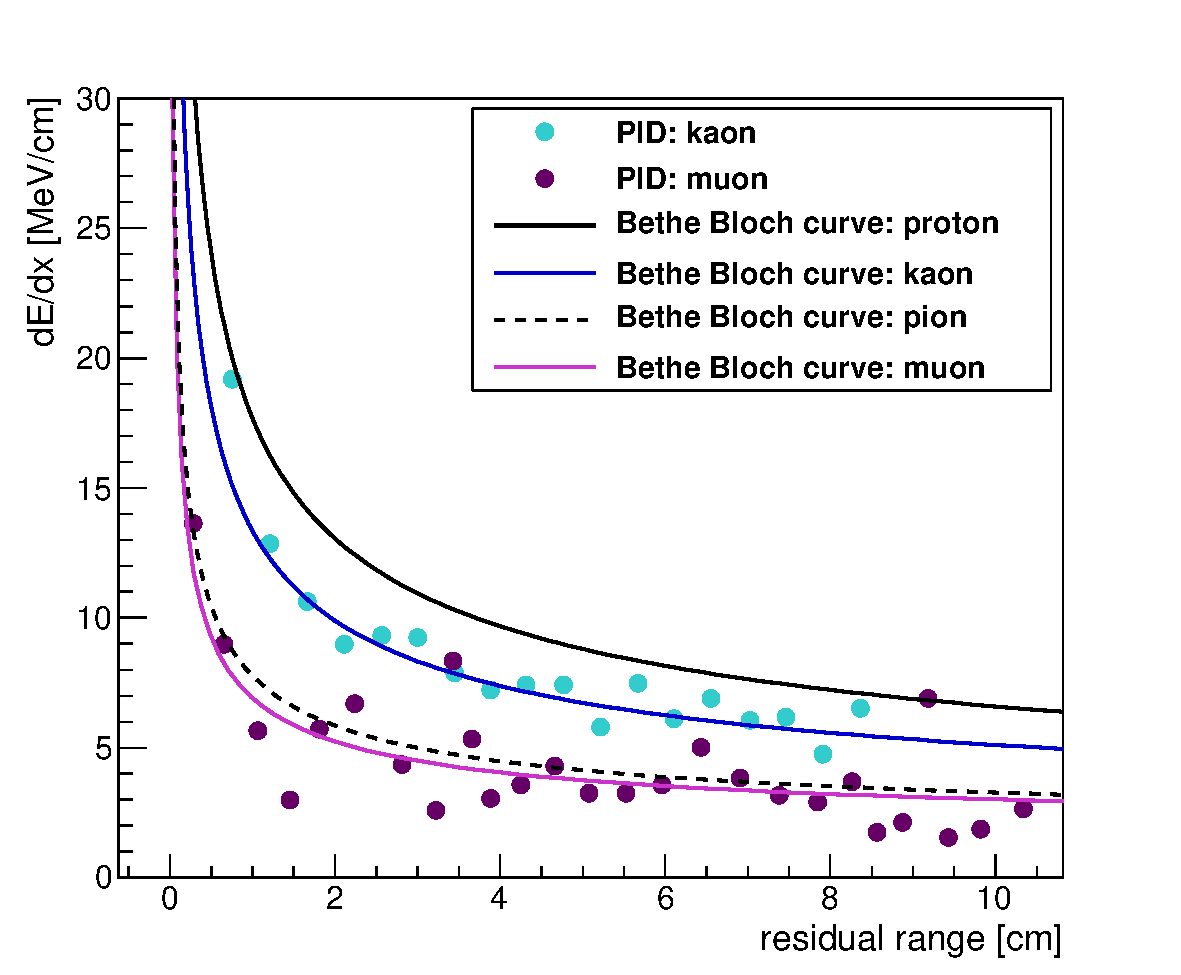
\includegraphics[width=0.8\textwidth]{Fig14d.pdf}
%\caption[$dE/dx$ profile of decaying kaon in the ICARUS CNGS run]
%        {Measurements of $dE/dx$ versus residual range for signals
%          associated with the kaon track in Figure~\ref{fig:icaruskaon} (cyan points) and the decay muon
%          (magenta points).  Overlaid are the expected $dE/dx$ profiles for the
%          two particle identities~\cite{Antonello:2012hu}. }
%\label{fig:pdkdedx}
%\end{figure}
%One variant of this background source occurs for the case where the
%pion decays in flight.  Two experimental handles on this background
%can be immediately identified.  First is the deviation from the
%expected $dE/dx$ profile for a kaon, which will be more dramatic than
%in the case of the stopping pion.  Second is the correlation of the
%direction of the decay muon with that of the pion, which is absent in
%the decay of a particle at rest.  Assessment of the cumulative impact
%of event rejection based on these features is under study.  However,
%the decaying kaon observed in the ICARUS CNGS run displayed in 
%Figure~\ref{fig:icaruskaon} can be used to give a sense of the 
%$\pi/K$ discrimination possible in a LArTPC via $dE/dx$.   
%In Figure~\ref{fig:pdkdedx}, the measurements
%of $dE/dx$ versus residual range for the anode wires registering
%signals from the kaon and muon tracks in this event are plotted
%against the expected $dE/dx$ profiles~\cite{Antonello:2012hu}. The
%data from the kaon track (cyan points) agree very well with the
%expected $dE/dx$ profile (blue curve) and are quite distinguishable
%from the expected pion profile (dashed curve).
%
%\textbf{\boldmath Event reconstruction pathologies:}
%While consideration of rare event topologies in atmospheric-neutrino 
%interactions is important, it will be equally important to understand 
%ways in which more typical events might be misreconstructed so as 
%to mimic nucleon decay processes.  For example, a quasi-elastic 
%$\nu_\mu$-CC interaction will produce a muon and a recoil
%proton from a common vertex.  However, it may be possible to interpret 
%the vertex as the kink associated with the decay of a stopping kaon, 
%where the proton track is confused with a kaon traveling in the opposite 
%direction.  Tools are still under development to be able to understand 
%the degree to which this possibility poses a potential background.  
%Naively, the $dE/dx$ profile of the proton as a function of residual range 
%will not match the time-reversed version of this for a kaon, 
%and distributions of kinematic quantities will be 
%distinct.  Additionally, such a background will only affect 
%the portion of the $p\to K^+\overline{\nu}$ analysis focused 
%on $K^+\to \mu^+\nu$; other $K^+$ decays will be immune to this 
%pathology.  
%
%The point of this example is to illustrate that although the 
%exquisite performance characteristics of the LArTPC technique 
%enables unambiguous identification of nucleon decay signatures, 
%an extensive program of detailed analysis will be required 
%to fully exploit these capabilities.
%
%\textbf{Conclusions on atmospheric-neutrino backgrounds:}
%The above examples suggest that it will be possible to demonstrate 
%the desired level of suppression of atmospheric-neutrino background 
%without undue reliance on simulations 
%via a combination of arguments based on existing experimental data 
%(from SK proton decay searches, as well as data from various 
%sources on exclusive and inclusive neutrino-interaction processes 
%that yield rare topologies), physics considerations, and detailed 
%analysis of anticipated detector response.  For the latter, 
%ongoing DUNE event-reconstruction efforts will play a role with 
%simulated atmospheric-neutrino samples.  Additionally, useful 
%input is expected to come in over the short/intermediate term 
%from analyses of LArTPC data from ArgoNeuT, SBND, MicroBooNE and 
%the proposed LArIAT.
%Finally, while the state of neutrino flux and interaction models 
%is already quite advanced, vigorous theoretical work is ongoing 
%to improve these further, exploiting existing data from neutrino 
%and electron-scattering experiments.  In particular, kaon production 
%in neutrino interactions in relevant energy ranges is receiving 
%renewed attention~\cite{gallagher-private}.
%%\fixme{if we want to cite something to support this last claim about theoretical work, we could cite H. Gallagher, private communication, although I'm sure Hugh has some suggestions for references to cite.}
%\clearpage
%%%%%%%%%%%%%%%%%%%%%%%%%%%%%%%%%%%%%%%%%%%%%%%%%%%%%%%%%%%%%%%%%
\subsection{\boldmath Summary of Expected Sensitivity to Key Nucleon Decay Modes}
%\section{\boldmath Expected Sensitivity to $p \rightarrow K^+ \overline{\nu}$}

Based on the expected signal efficiency and the upper limit on the
background rates estimated in Section~\ref{sec:pdk:background-rej}, 
the expected limit on the proton
lifetime as a function of running time in DUNE for $p \rightarrow K^+
\overline{\nu}$ is shown in 
Figure~\ref{fig:kdklimit}. 
\begin{figure}[!htb]
\centering
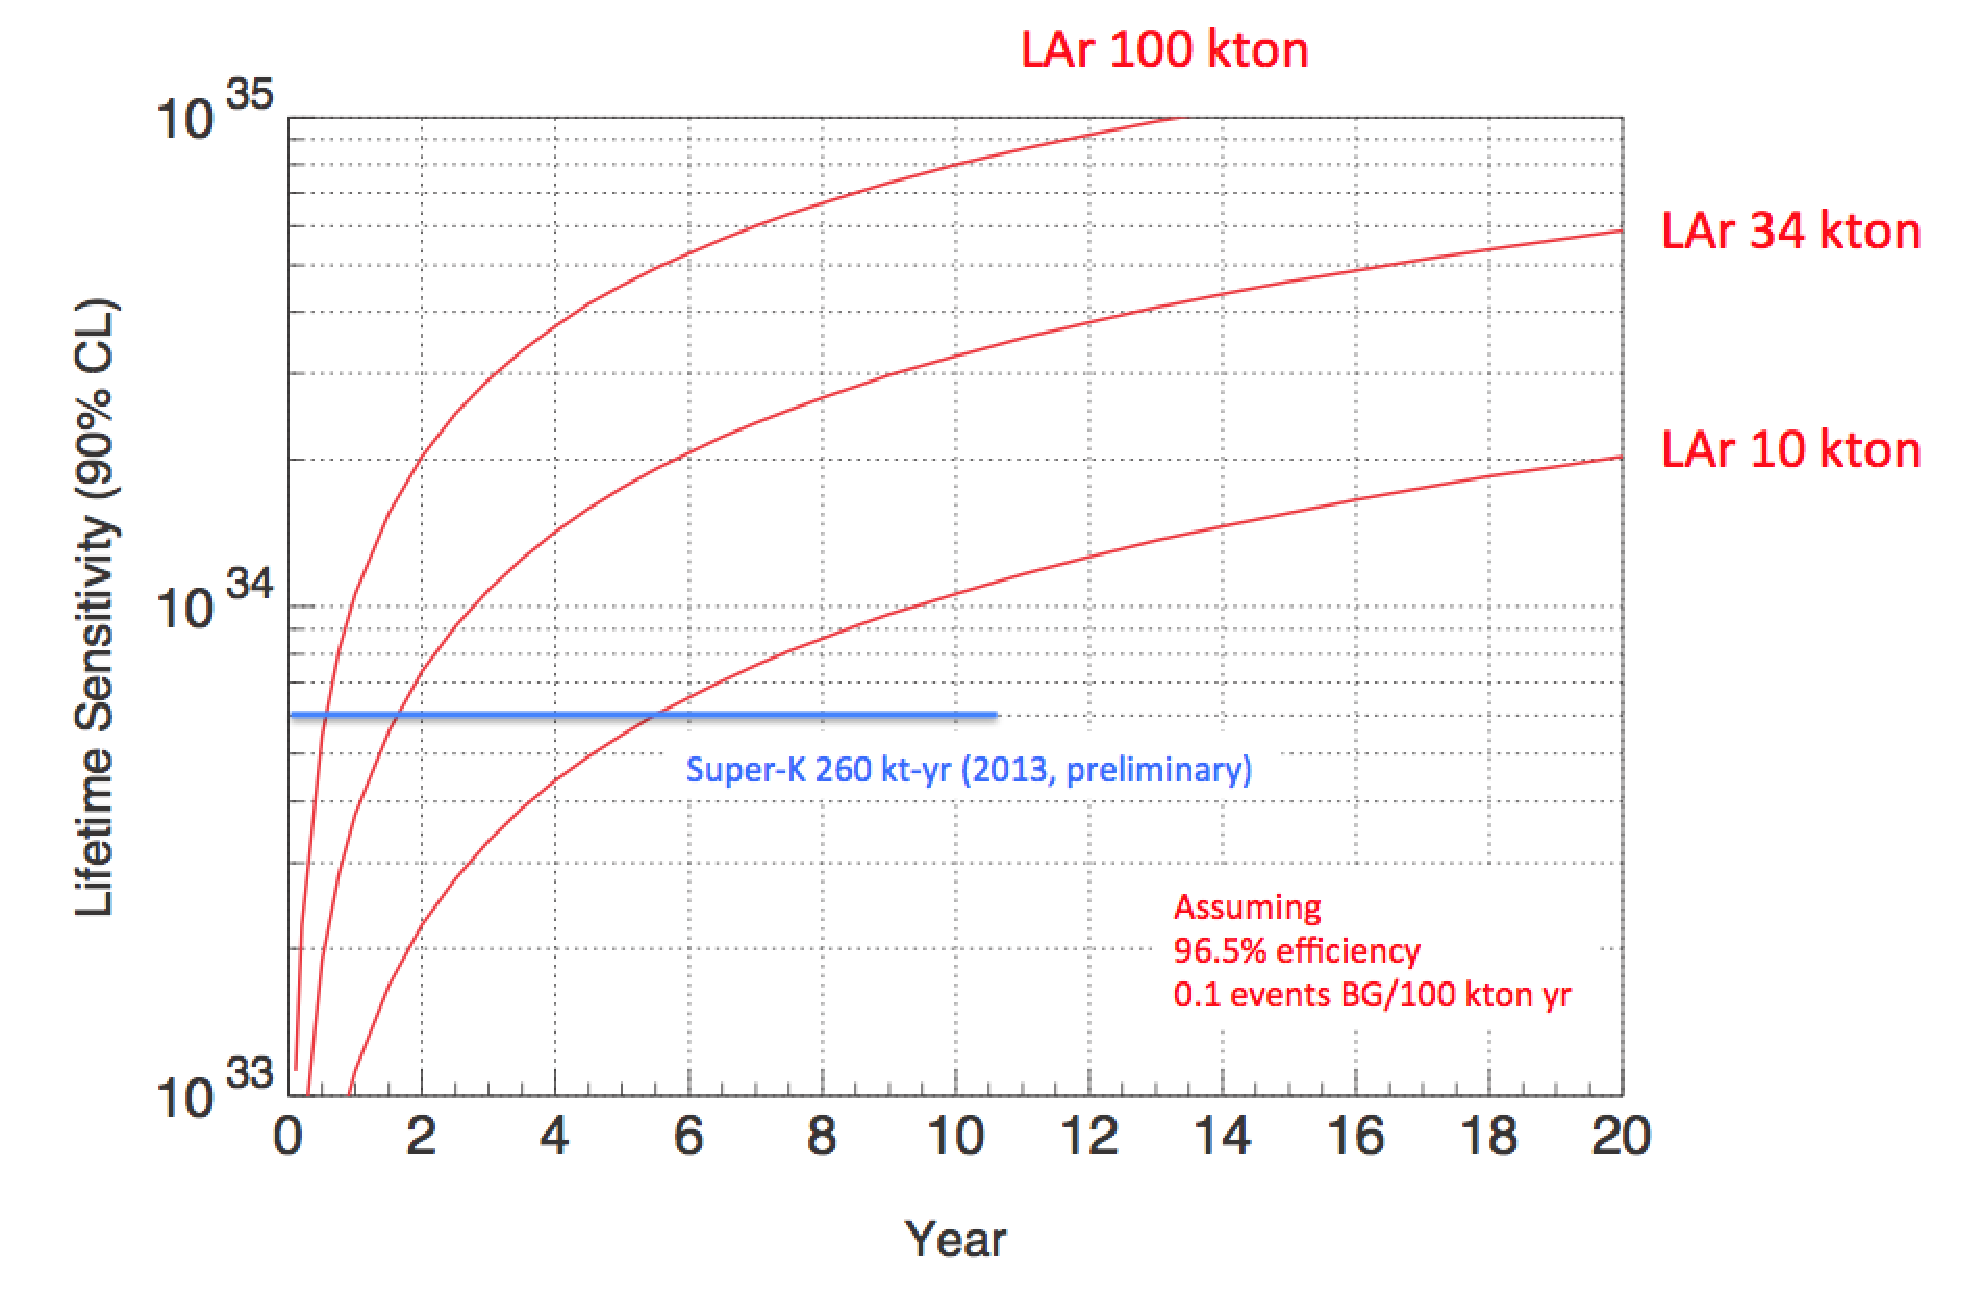
\includegraphics[width=0.8\textwidth]{pdecay_kearns_pac2013.pdf}
\caption[Proton decay lifetime limit for $p \rightarrow K^+ \overline{\nu}$
  versus time]{Proton decay lifetime limit for $p
  \rightarrow K^+ \overline{\nu}$ as a function of time for
  underground LArTPCs of fiducial masses 10, 34 and 100~kt.
  For comparison, the current limit from SK is also shown.
  The limits are at 90\% C.L., calculated for
  a Poisson process including background, assuming that the detected events
  equal the expected background.}
\label{fig:kdklimit}
\end{figure}
%
%\begin{introbox}
Figure~\ref{fig:kdklimit} demonstrates that 
to improve the current limits on
the $p \rightarrow \overline{\nu} K^+$, set by \superk, significantly
beyond that experiment's sensitivity, 
a LArTPC
detector of at least 10~kt, installed deep underground, is needed.
A \ktadj{34} detector will improve the current limits by an order of
magnitude after running for two decades.  Clearly a larger detector
mass would improve the limits even more in that span of time.
%\end{introbox}

While the background rates are thought to be no higher than those assumed 
in generating the above sensitivity projections, it is possible to estimate 
the impact of higher rates.  For $p\to K^+\overline{\nu}$, 
Table~\ref{tab:pdecay-bgvariation} shows a comparison of the 
$90\%$ CL lower bounds on proton lifetime for an exposure  of \SI{340}{\ktyr} 
assuming the nominal 1.0 per  \SI{}{\Mtyr} background rate with the 
corresponding bounds for a rate that is ten times higher, as well as for 
a fully background-free experiment.
%\fixme{Make sure we get rid of one of these tables!!}
%
%\begin{table}[!htb]
%\caption{Compare format
%        }
%\begin{center}
%\begin{tabular}{$l^c} %{ll} 
%\toprule
%\rowcolor{\ChapterBubbleColor}
%Background Rate & Expected Partial Lifetime \\ \toprowrule
%0 events/Mt-yr    & $3.8 \times 10^{34}$ years  \\ \colhline
%1 events/Mt-yr    & $3.3 \times 10^{34}$ years  \\ \colhline
%10 events/Mt-yr    & $2.0 \times 10^{34}$ years  \\
%\bottomrule
%\end{tabular}
%\end{center}
%\label{tab:pdecay-bgvariation}
%\end{table}
%
While a factor of ten increase in the background would hurt the 
sensitivity, useful limits can still be obtained.  As stated 
above, however, there is good reason to believe such a case 
is highly unlikely.
%

%
\begin{cdrtable}[Sensitivity for $p\to K^+\overline{\nu}$ with different background rates]{lc}{pdecay-bgvariation}{The impact of different assumed background rates on the expected 
         $90\%$ CL lower bound for the partial proton lifetime for 
         the $p\to K^+\overline{\nu}$ channel, for a \ktadj{34} detector 
         operating for ten years.  The expected background rate is 
         one event per  \SI{}{\Mtyr}.  Systematic uncertainties are not included 
         in these evaluations.}
Background Rate & Expected Partial Lifetime Limit\\ \toprowrule
0 events/\SI{}{\Mtyr}    & $3.8 \times 10^{34}$ years  \\ \colhline
1 events/\SI{}{\Mtyr}    & $3.3 \times 10^{34}$ years  \\ \colhline
10 events/\SI{}{\Mtyr}    & $2.0 \times 10^{34}$ years  \\
\end{cdrtable}


%%%%%%%%%%%%%%%%%%%%%%%%%%%%%%%%%%%%%%%%%%%%%%%%%%%%%%%%%%%%%%%%
%%%%%%%%%%%%%%%%%%%%%%%%%%%%%%%%%%%%%%%%%%%%%%%%%%%%%%%%%%%%%%%%
%\section{Summary of Expected Sensitivities}
%
Sensitivities have been computed for some of the other
decay channels listed in Table~\ref{tab:pdecay}. The limits that could
be obtained from an DUNE \ktadj{34} detector in ten years of running as
compared to other proposed future experiments and theoretical
expectations are shown in Figure~\ref{fig:nnn13}.
\begin{figure}[!htb]
\centering
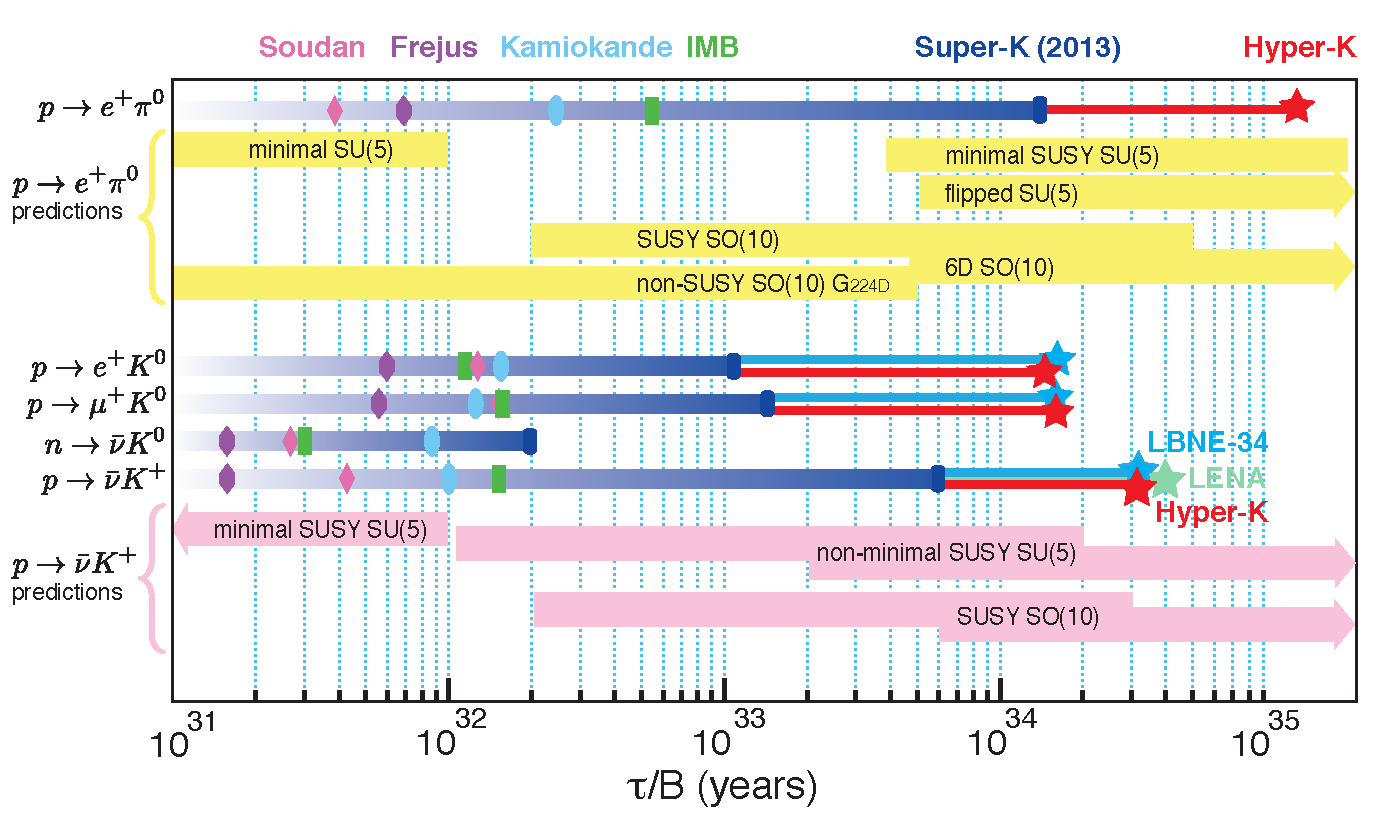
\includegraphics[width=\textwidth]{sklimits_compare_theory_2013_hklenalbne.pdf}
\caption[Proton decay lifetime limits achievable by \ktadj{34} DUNE;
comparison to others]{Proton decay
  lifetime limits that can be achieved by the DUNE \ktadj{34} detector compared
  to other proposed future experiments.  The limits are at 90\% C.L.,
  calculated for a Poisson process including background, assuming that
  the detected events equal the expected background.}
\label{fig:nnn13}
\end{figure}



\section{Atmospheric Neutrinos}
\label{sec:physics-atmpdk-atmnu}

Atmospheric neutrinos are a unique tool to study neutrino oscillations: they 
contain all flavors of neutrinos and anti-neutrinos, are very sensitive to 
matter effects and to both $\Delta m^2$, and cover a wide range of L/E. In principle, 
all oscillation parameters could be measured, with high complementarity to 
measurements performed with a neutrino beam. In addition, atmospheric 
neutrinos are available all the time, in particular before the beam becomes 
operational. Atmospheric neutrinos also provide a laboratory in which to search 
for exotic phenomena where the dependence of the flavor-transition and survival 
probabilities on energy and path length can be defined. The DUNE far detector, 
with its large mass and the overburden to protect it from backgrounds, is an 
ideal tool for these studies. In the following, we will focus on the 
measurement of the oscillation parameters where the role of atmospheric neutrinos is 
most important. 

The sensitivity to oscillation parameters has been evaluated with a 
dedicated simulation, reconstruction and analysis chain. 
% HG:  We need references here
The fluxes, after 
oscillation, of each neutrino species at the far detector location were 
computed. Interactions in the LAr medium were simulated with the GENIE event 
generator. Detection thresholds and energy resolutions based on full 
simulations were applied to the outgoing particles, to take into account 
detector effects. Events were classified as Fully Contained (FC) or 
Partially Contained (PC) by placing the vertex at a random position inside the 
detector and tracking the lepton until its edges. The number of events expected 
for each flavor and category is summarized in Table~\ref{tab:atmos_rates}.

%
\begin{table}[!htbp]
\caption[Atmospheric-neutrino event rates]
        {
         Atmospheric-neutrino event rates including oscillations in \SI{350}{\ktyr} 
         with a LArTPC, fully or partially contained in the detector fiducial volume. 
        }
\begin{center}
\begin{tabular}{$L^c} %$ 
\toprule
\rowtitlestyle
Sample   &  Event Rate \\ \toprowrule
fully contained electron-like sample   &14,053 \\ \colhline
fully contained muon-like sample       &20,853 \\ \colhline
partially contained muon-like sample   & 6,871 \\ \colhline
\bottomrule
\end{tabular}
\end{center}
\label{tab:atmos_rates}
\end{table}
%

Figure shows the expected L/E distribution for high-resolution muon-like 
events from a \SI{350}{\ktyr} exposure. The data provide excellent resolution of the 
first two oscillation nodes, even when taking into account the expected statistical uncertainty.
In performing oscillation fits, the data in each flavor/containment category are 
binned in energy and zenith angle. 

\begin{figure}[!htb]
\centering
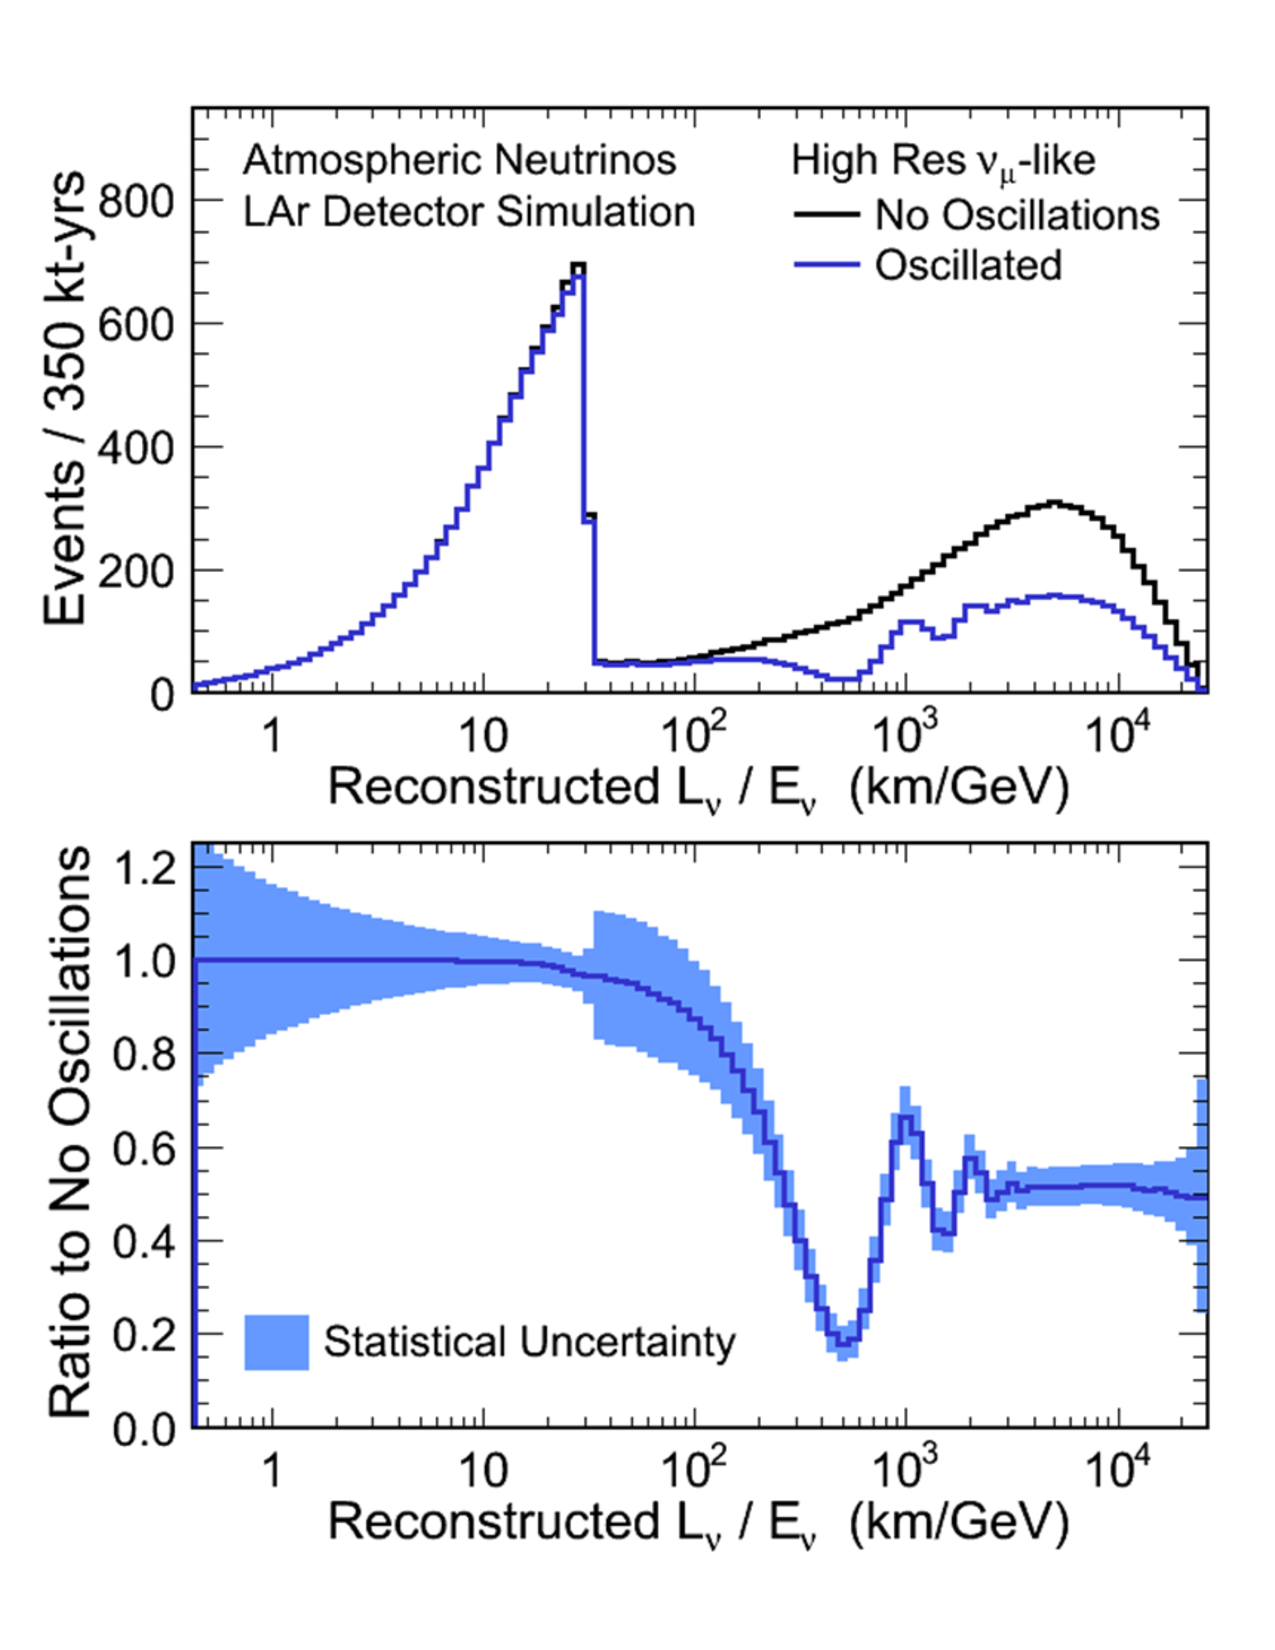
\includegraphics[width=0.6\textwidth]{atm_spectrum_LoverE.pdf}
\caption[Reconstructed L/E Distribution of `High Resolution' Atmospheric Neutrinos]
{Reconstructed L/E Distribution of `High Resolution'
$\mu$-like atmospheric neutrino events in a \SI{350}{\ktyr} exposure with and
without oscillations (top), and the ratio of the two (bottom), with the
shaded band indicating the size of the statistical uncertainty.}
\label{fig:lovere}
\end{figure}

\subsection{Sensitivity to Mass Hierarchy}

When neutrinos travel through the Earth, the MSW resonance influences 
electron neutrinos in the few-GeV energy range. More precisely, the resonance 
occurs for $\nu_e$ in the case of normal mass hierarchy (NH, $\Delta m^2_{23} >0$), and for 
anti-νe in the case of inverted mass hierarchy (IH, $\Delta m^2_{23} <0$). This is 
illustrated in Figure~\ref{atm_e_zenith}. 

\begin{figure}[!htb]
\centering
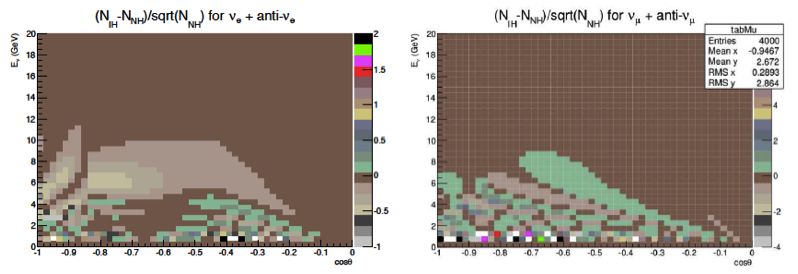
\includegraphics[width=0.95\textwidth]{atm_e_zenith.png}
\caption[Zenith Angle vs. Energy For Atmospheric Neutrinos]
{Statistical significance of the difference in expected event rates for NH and IH for 
muon-type events (left) and electron-type events (right), as a function of neutrino
energy and zenith angle.}
\label{fig:atm_e_zenith}
\end{figure}

The MH sensitivity can be greatly enhanced if neutrino and antineutrino events can be 
separated. The DUNE detector will not be magnetized; however, its high-resolution 
imaging offers possibilities for tagging features of events that provide statistical 
discrimination between neutrinos and antineutrinos. For the sensitivity calculations 
that follow, two such tags were included: a proton tag and a decay electron tag. 
%The 
%reconstructed zenith angle distribution for different event categories is shown in Figure~\ref{fig:atmzenith}.

%\begin{figure}[!htb]
%\centering
%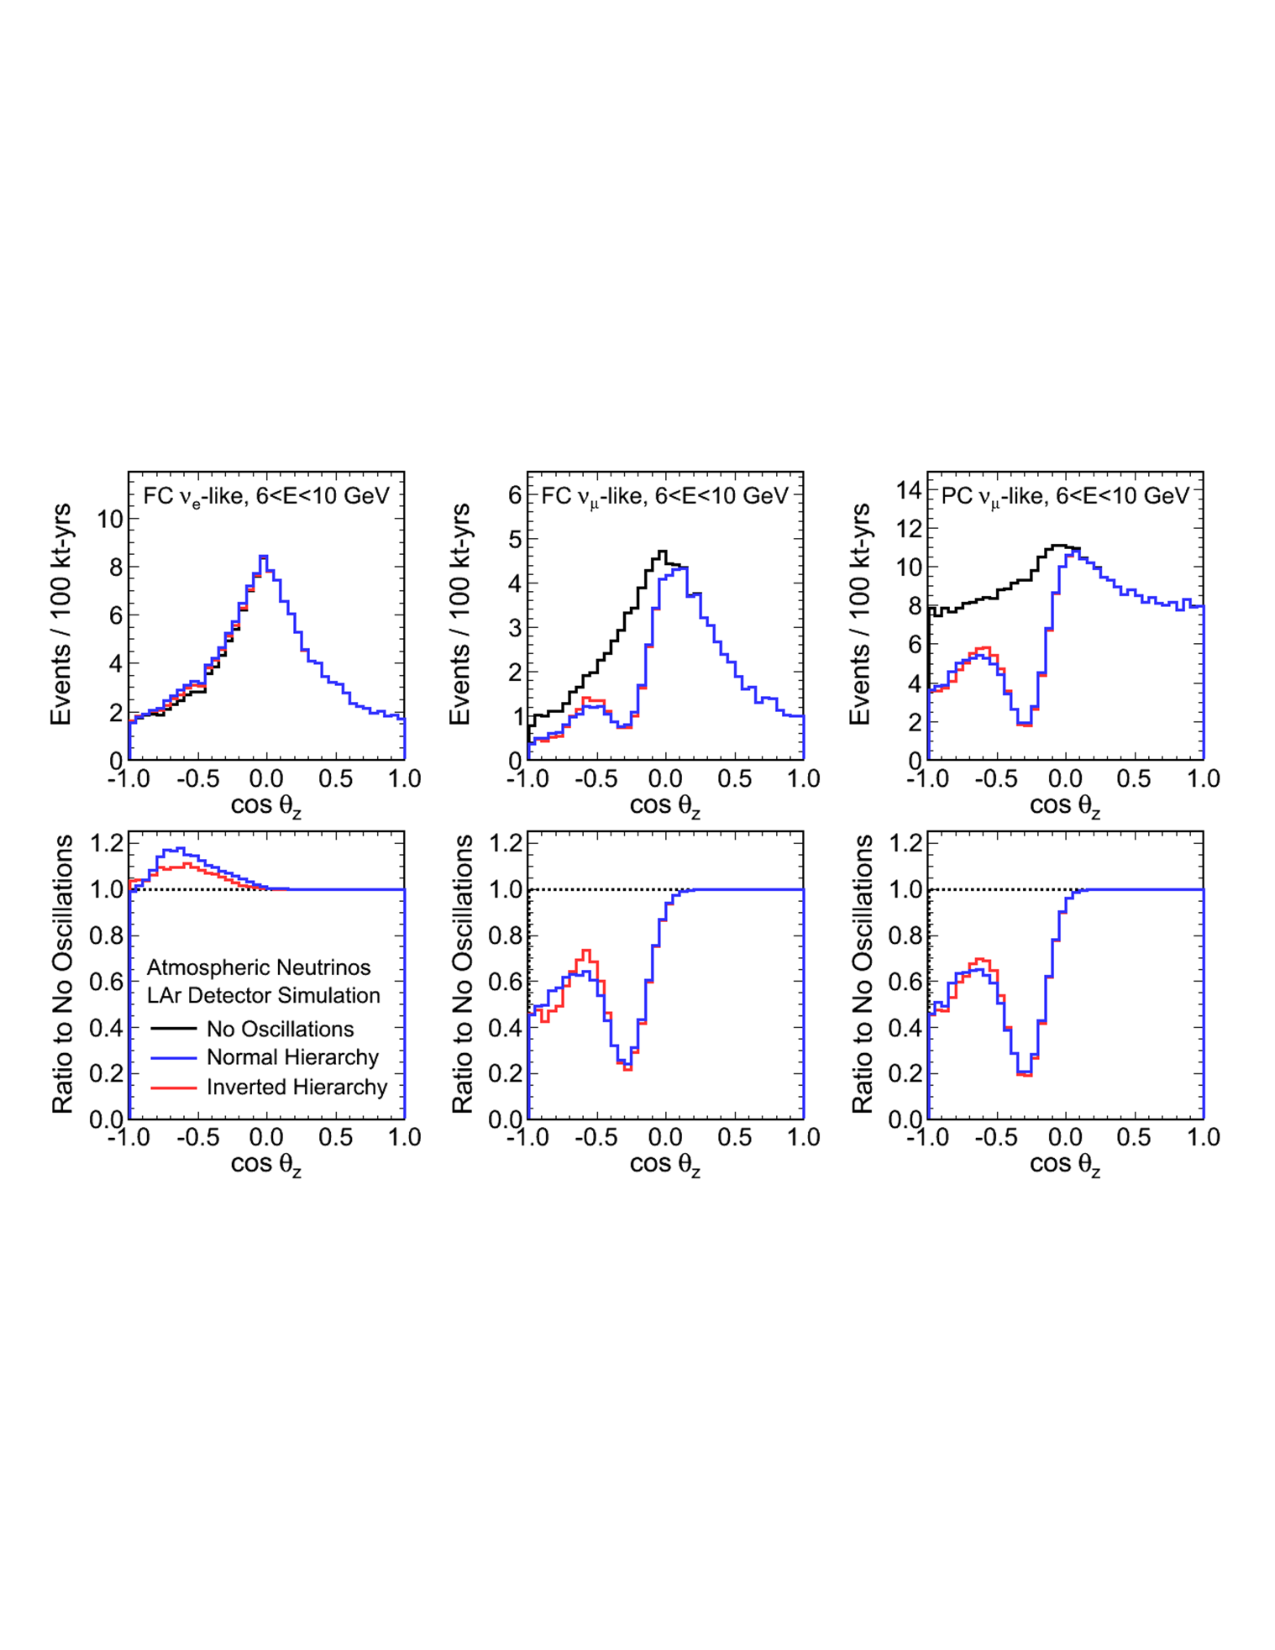
\includegraphics[width=0.95\textwidth]{atm_event_spectra_zenth_6to10gev.pdf}
%\caption[Reconstructed Zenith Angle Distributions for Atmospheric Neutrinos]
%{Reconstructed zenith angle distributions for 6 to 10-GeV events in the different FC and 
%PC samples. Top plots show the expected distributions for no oscillations (black), oscillations with 
%normal (blue), and inverted (red) hierarchy. Bottom plots show the ratio of the normal and inverted 
%expectations to the no-oscillation distributions for each category.}
%\label{fig:atmzenith}
%\end{figure}

Figure~\ref{fig:atm_mh} shows the MH sensitivity as a function of the fiducial exposure. 
Over this range of fiducial exposures, the sensitivity goes essentially as the square 
root of the exposure, indicating that the measurement is not systematics-limited. 
Unlike for beam measurements, he sensitivity to MH with atmospheric neutrinos is 
nearly independent of the CP violating phase.

\begin{figure}[!htb]
\centering
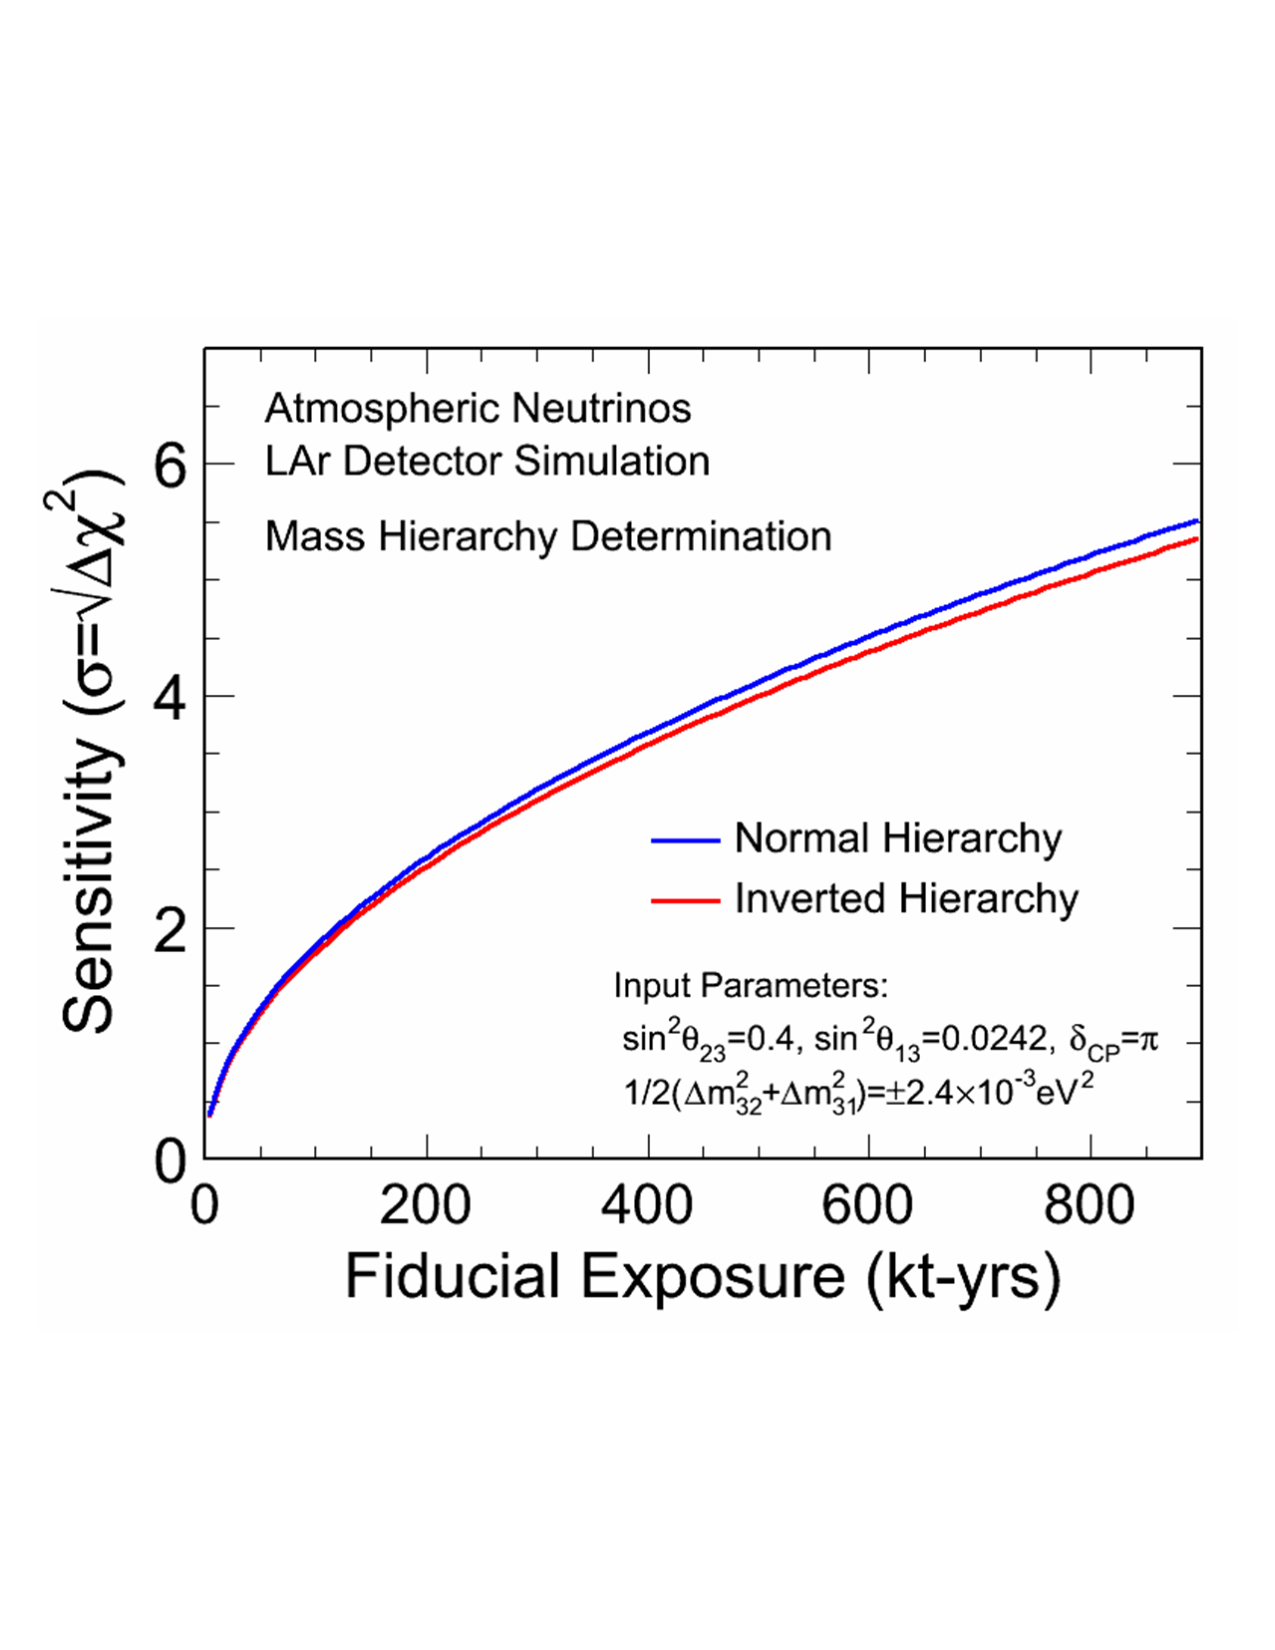
\includegraphics[width=0.40\textwidth]{atm_mh_vs_exposure.pdf}
\caption[MH Sensitivity vs. Exposure for Atmospheric Neutrinos]
{Sensitivity to mass hierarchy using atmospheric neutrinos as a function of fiducial 
exposure in a liquid argon detector.}
\label{fig:atm_mh}
\end{figure}

\subsection{Sensitivity to the $\theta_{23}$ octant}

In the two-flavour approximation, neutrino oscillation probabilities depend on 
$\sin^2(2θ)$, which is invariant when changing $\theta$ to $\pi/2-\theta$. The octant 
degeneracy remains for $\theta_{23}$ in the leading order terms of the full 
three-flavor oscillation probability, making it impossible to determine whether $\theta_{23}< \pi/4$ or 
$\theta_{23}> \pi/4$. Accessing full three-flavor oscillation with atmospheric neutrinos 
will give a handle to solve the ambiguity.

%The sensitivity to the $\theta_{23}$ octant is shown in Figure~\ref{fig:atm_octant}. 
With the nominal exposure of \SI{340}{\ktyr}, DUNE will be able to distinguish between 
octants at 3$\sigma$ significance, based on atmospheric data alone, for true values of [quantify], 
for any value of $\delta_{CP}$.

%\begin{figure}[!htb]
%\centering
%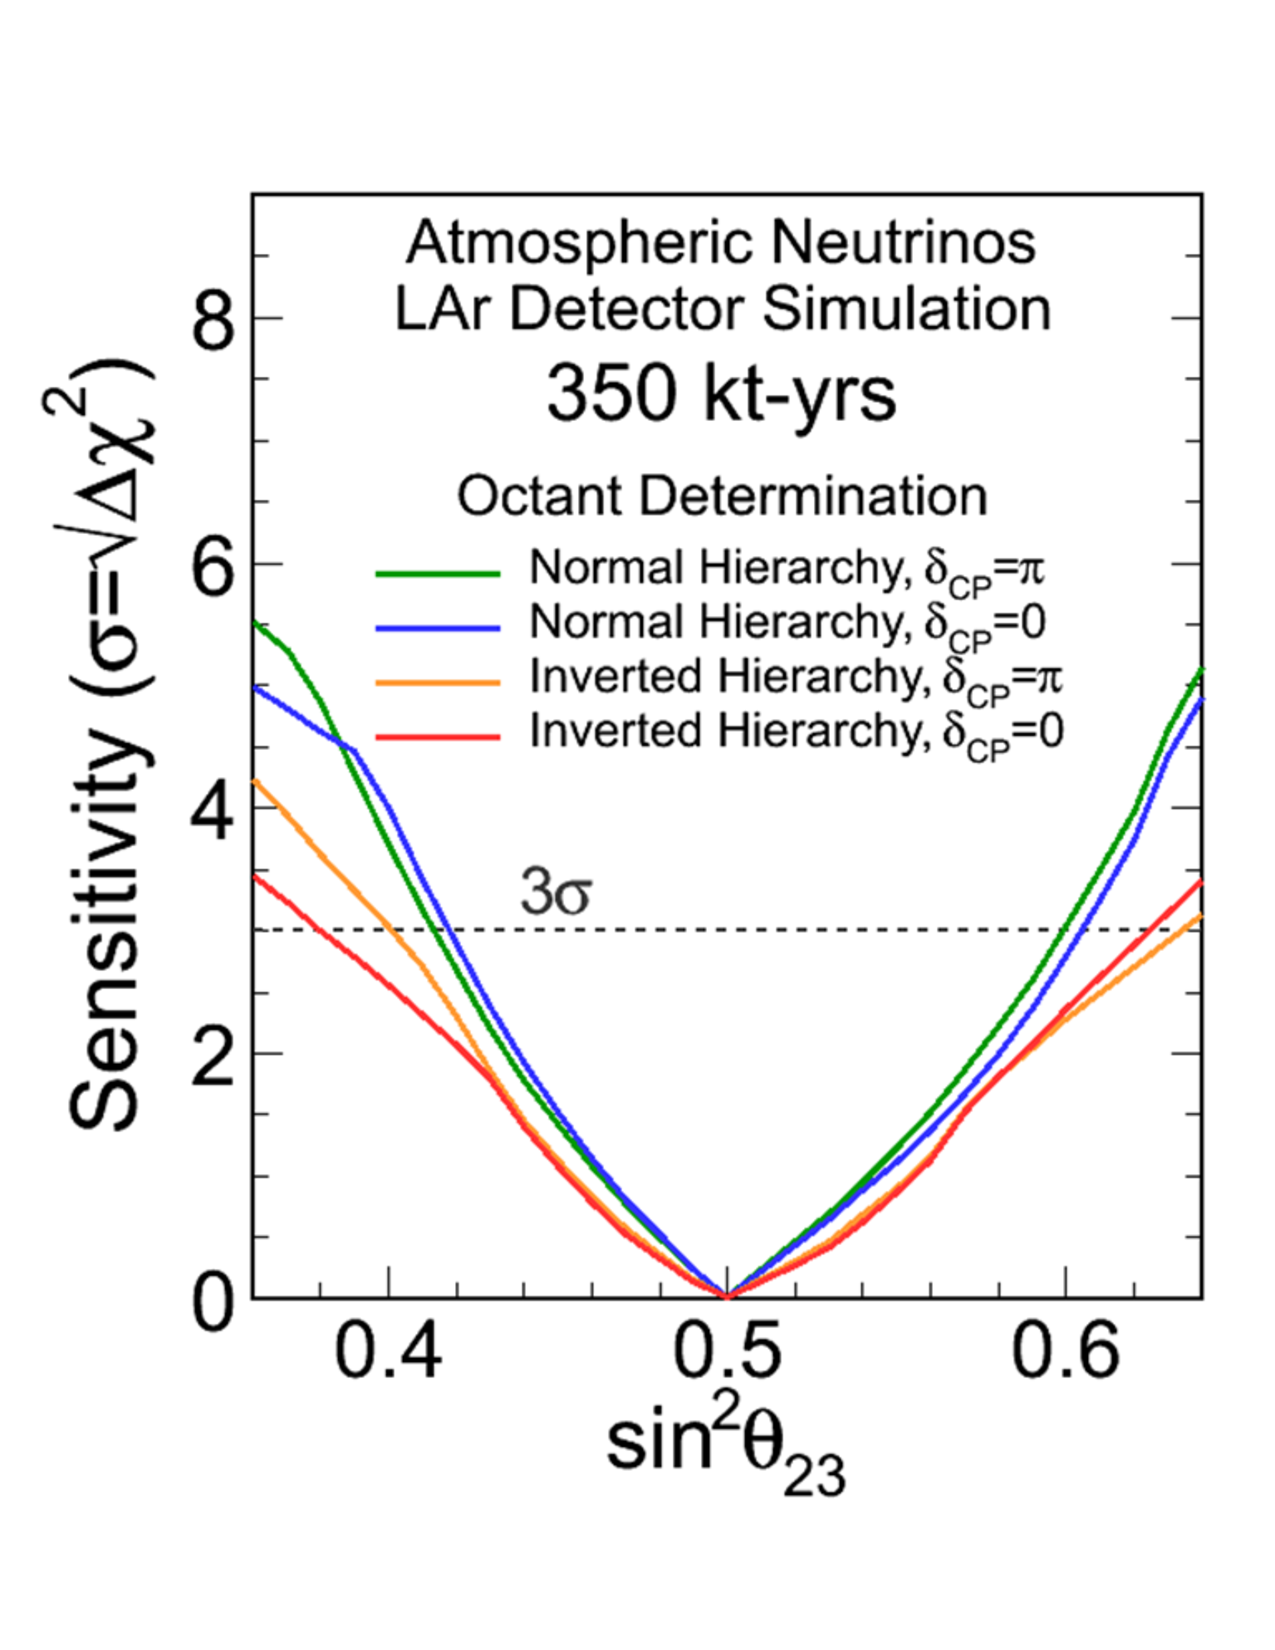
\includegraphics[width=0.60\textwidth]{atm_octant_sens.pdf}
%\caption[Octant Sensitivity for Atmospheric Neutrinos]
%{Sensitivity to $\theta_{23}$ octant for atmospheric neutrinos.}
%\label{fig:atm_octant}
%\end{figure}

%The sensitivity of atmospheric neutrinos to CPV is quite limited and will not reach 
%$3\sigma$ with the nominal exposure, as shown in Fig. 4.27.

These analyses will provide a complementary approach to beam neutrinos.   Atmospheric neutrinos can 
help to lift degeneracies that can be present in beam analyses, for instance, through the fact that the 
MH sensitivity is essentially independent of $\delta_{CP}$.   Atmospheric neutrino data will be acquired 
even in the absence of the beam, and will provide a useful sample for the development of 
reconstruction software and analysis methodologies.  

\section{Detector Requirements}
\label{sec:physics-atmpdk-detector-requirements}
